\chapter{Downloading and Installing Salome}
\thispagestyle{empty}
\label{sec:chap10}
\newcommand{\LocCHtenfig}{\Origin/CHAPTERS/chap10/figures}

Salome is a Free and Open Source  CAD (Computer Aided Drawing), Meshing and Visualization Software for Numerical simulation. 
We can Create/modify, import/export (IGES, STEP, BREP), repair/clean CAD models and Mesh CAD models, edit mesh, check mesh quality, 
import/export mesh (MED, UNV, DAT, STL) using Salome. In this chapter we will learn how to download and intall Salome in any Operating system.

\section{Download Salome}

Open your browser and in the address bar type the url given below, \newline

\centering \textbf{www.salome-platform.org} \newline

\flushleft To Download Salome the user needs to create a account on the salome site. To do this on the left hand side of the salome screen website
scroll down to the bottom of the \textbf{Navigation} bar, Fig \ref{navi}, where you can see the new user option. Click on it and enter the required
personal details. \newline
\flushleft After you enter the details click on the register button at the bottom as shown in, Fig \ref{details}. Once done you will be directed 
to a screen showing that you have been registered. This also states thatv once you have done with registration you have to login to your email. Now 
open the mail sent by Salome and click on the link shown in Fig, \ref{link}. This link will direct you to a window where you need to set your password
for your Salome account. Enter the password and confirm it and press set my password button, Fig \ref{pass}. After this it will direct you to a window
which says your password has been set successfully. You may now login with your username and password. \newline

\flushleft In the Navigation bar click on Downloads after which you will be directed to a page which will show various bianaries for various Linux
distributions. You can choose according to your Operating System and 32/64 bit size. Since in this book we are working on a 64 bit platform we
will download Linux Debian 7 64-bits binary, Fig \ref{binary}. Click on it and Save the file. Downloading may take some time due to the large file size.
After this scroll down to Universal Binaries and click on the \textbf{Linux 64-bits} to download it. Note that 32-bit version of binaries are no
more supported for the latest version of Salome. \newline

\section{Installation}

Create a new folder in your home directory by the name Salome. Once these files are downloaded go to your Downloads folder and copy the tar file and a Self Extracting file and paste this inside your Salome folder. To extract the tar file right click on the tar file and select extract here. We can now see the extract wizard folder. \newline

Open a new terminal window and type in the path for the Installation Wizard folder in  the Salome folder of your home directory. \newline

\centering \textbf {cd /home/Salome/InstallationWizard\_7.6.0\_Debain\_64bits} \newline

\flushleft Type ls to view the content inside the file. An executable file by the name \textbf{runInstall} can be seen here. The Installation Wizard can be launched in two modes : GUI and Batch. The default installation settings can be overridden by using command line options. Each option has a short and a long notation. In the command line type : \newline

\centering \textbf{ ./runInstall [options]} \newline 

\flushleft Options include 

\begin{itemize}

\item -g / --gui : Runs the Installation Wizard in the GUI mode (this is the default mode).

\item -b / --batch : Runs the Installation Wizard in the terminal mode.

\end{itemize}

\flushleft Once the user has finished installation by either the GUI or Batch mode we now need to install the universal library. Since the binary is available in the same folder in the 
command terminal we can type : \newline 

\centering \textbf{ ./Salome-V7\_6\_0-LGPL-x86-64.run} and press enter \newline

\flushleft Enter the default path for the installation file. After this type N to use Salome in English.The installation prcocess now starts and might take a while. Close the terminal once this is done. Now you can see the Salome icon on your Desktop, Fig \ref{salome-icon}. Double click on this to open the Salome working window, Fig \ref{salome-win}. This brings us to the end of the chapter. In the next chapter we will learn more about how to create Geometries using Salome and using it for our OpenFOAM Simulation.



\begin{figure}[h]  
\centering
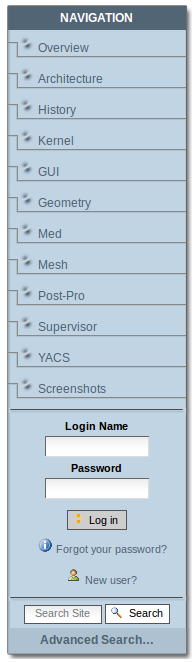
\includegraphics[scale=0.3]{\LocCHtenfig/navi.png}
\caption{Navigation Bar}
\label{navi}
\end{figure}

\begin{figure}[h]  
\centering
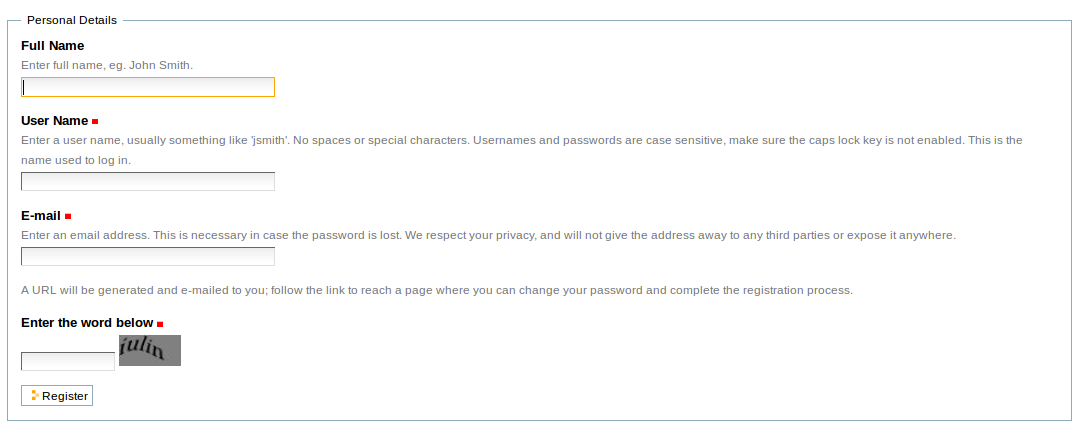
\includegraphics[scale=0.32]{\LocCHtenfig/details.png}
\caption{User Details}
\label{details}
\end{figure}

\begin{figure}[h]  
\centering
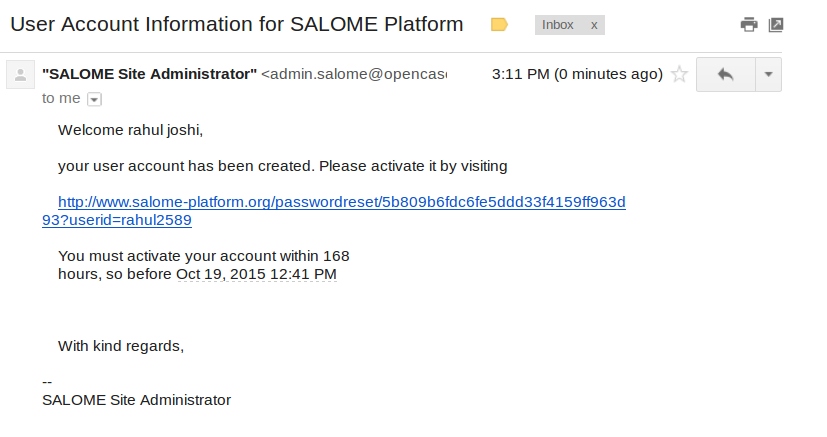
\includegraphics[scale=0.35]{\LocCHtenfig/link.png}
\caption{Salome Link}
\label{link}
\end{figure}

\begin{figure}[h]  
\centering
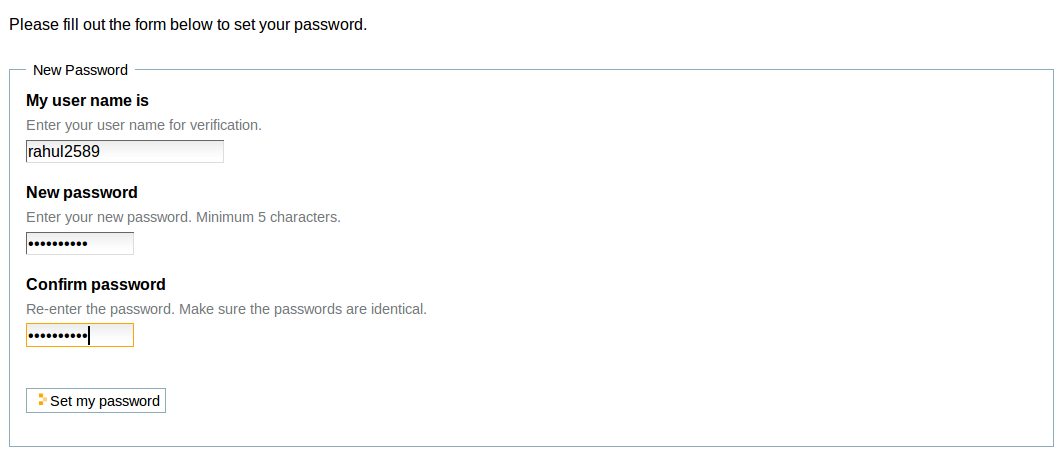
\includegraphics[scale=0.35]{\LocCHtenfig/pass.png}
\caption{Enter Password}
\label{pass}
\end{figure}

\begin{figure}[h]  
\centering
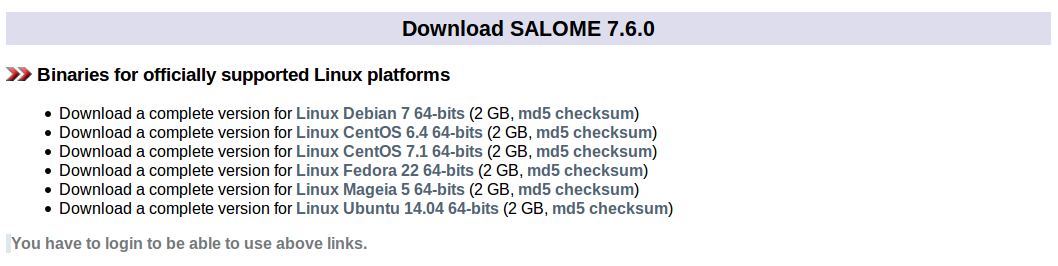
\includegraphics[scale=0.35]{\LocCHtenfig/binary.png}
\caption{Salome Linux 7 64 bit binary}
\label{binary}
\end{figure}

\begin{figure}[h]  
\centering
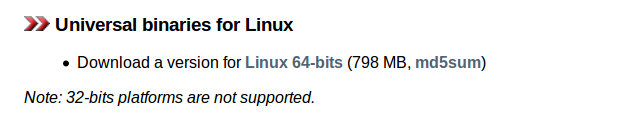
\includegraphics[scale=0.35]{\LocCHtenfig/universal.png}
\caption{Universal Binaries}
\label{univ}
\end{figure}

\begin{figure}[h]  
\centering
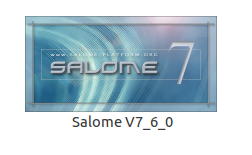
\includegraphics[scale=0.35]{\LocCHtenfig/salome-icon.png}
\caption{Salome icon}
\label{salome-icon}
\end{figure}

\begin{figure}[h]  
\centering
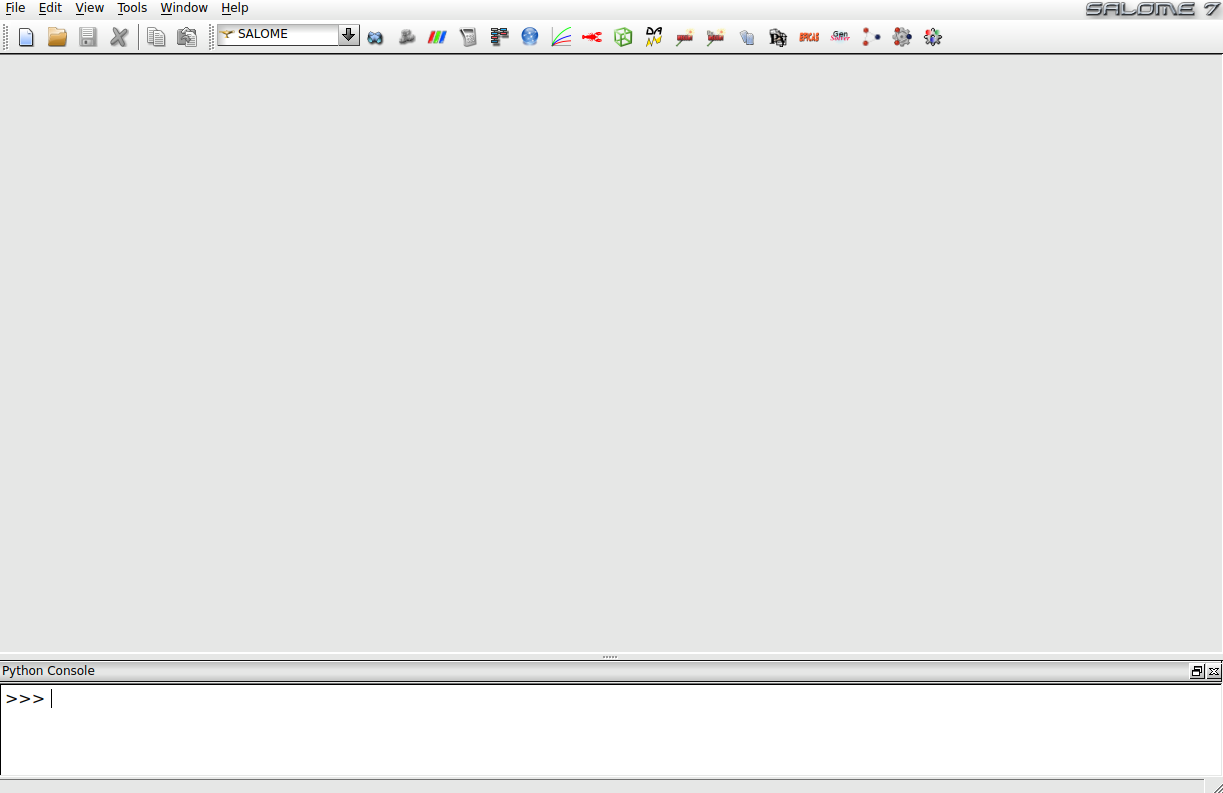
\includegraphics[scale=0.25]{\LocCHtenfig/salome-win.png}
\caption{Salome working window}
\label{salome-win}
\end{figure}
